\documentclass{article}
\usepackage{amsmath}
\usepackage{amssymb}
\usepackage{tikz}
\usetikzlibrary{patterns}

\begin{document}

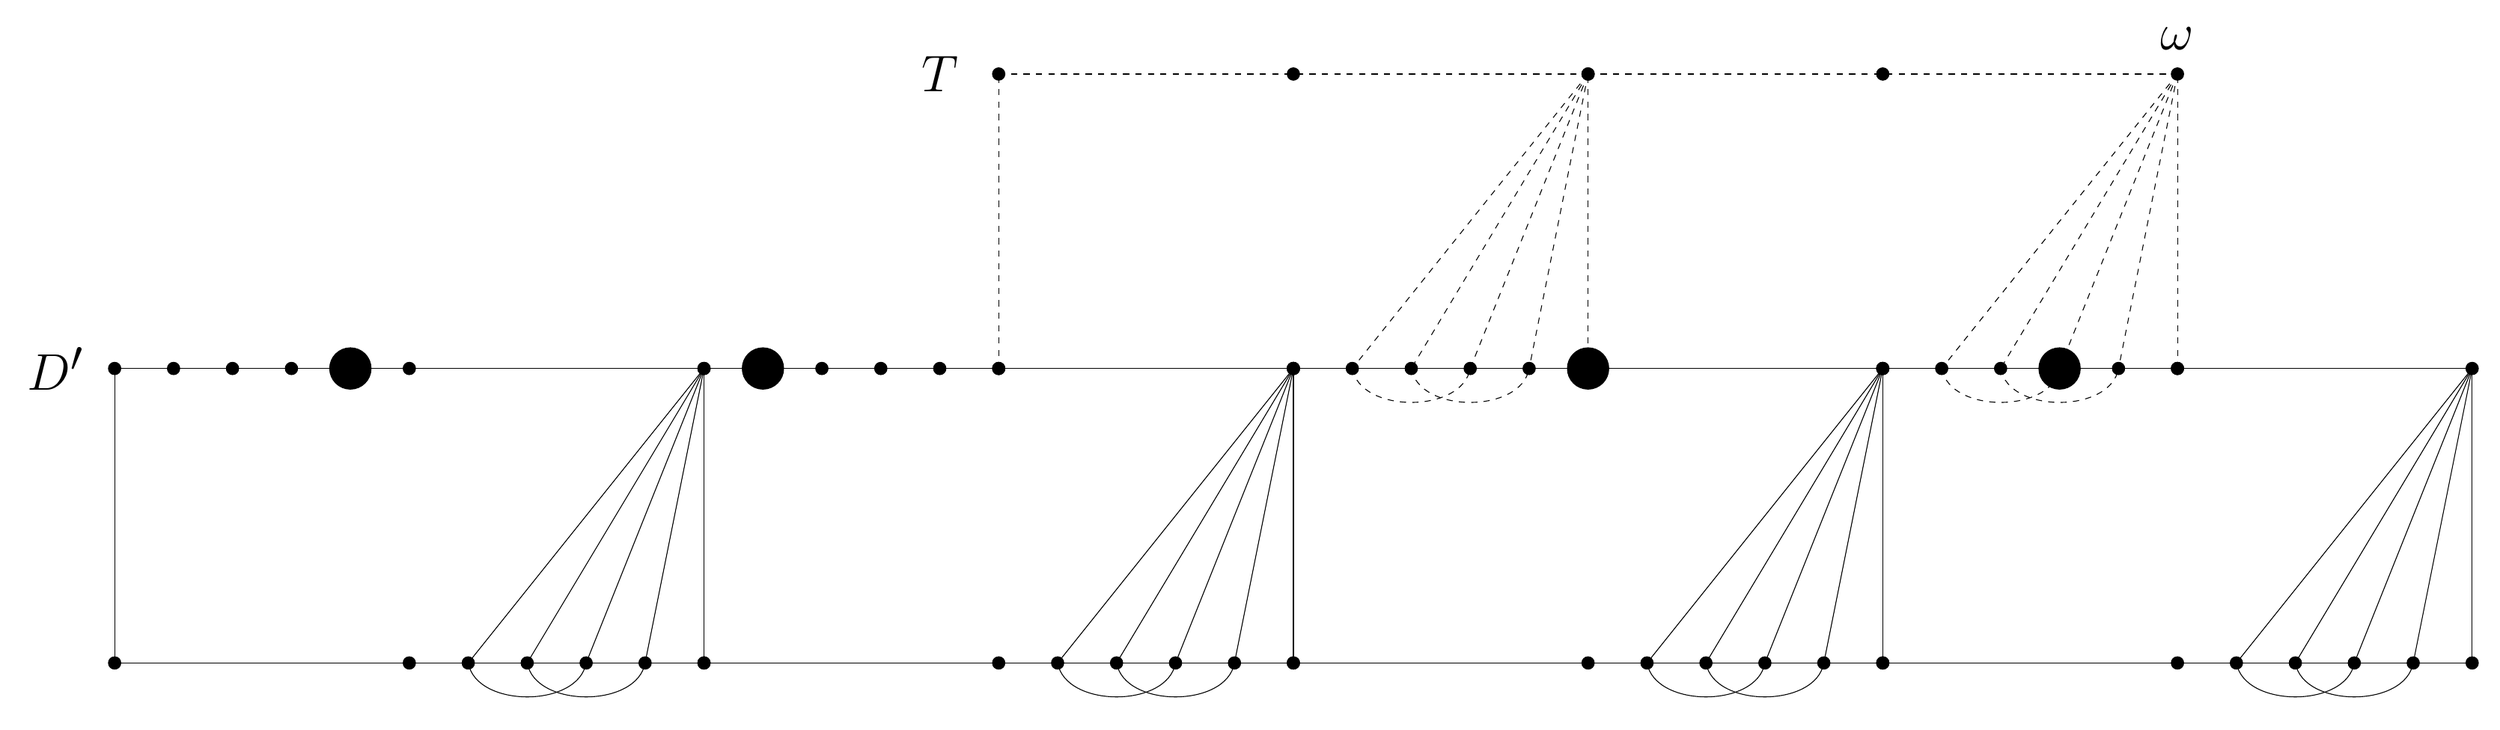
\begin{tikzpicture}
      \def\y{0}
      \foreach \x in {\y, 10 + \y, 20 + \y, 30 + \y} {
        \draw (\x, \y) -- (10 + \x, \y);
        \draw (\x, 5 + \y) -- (10 + \x, 5 + \y);
        \draw (\x, \y) -- (\x, 5 + \y);
        \draw (10 + \x, \y) -- (10 + \x, 5 + \y);

        \draw (10 + \x, 5 + \y) -- (6 + \x, \y);
        \draw (10 + \x, 5 + \y) -- (7 + \x, \y);
        \draw (10 + \x, 5 + \y) -- (8 + \x, \y);
        \draw (10 + \x, 5 + \y) -- (9 + \x, \y);
  
        \draw (6 + \x, \y) to[out = -80, in = -100] (8 + \x, \y);
        \draw (7 + \x, \y) to[out = -80, in = -100] (9 + \x, \y);
  
        \filldraw [black] (\x, \y) circle (3pt);
        \filldraw [black] (5 + \x, \y) circle (3pt);
        \filldraw [black] (6 + \x, \y) circle (3pt);
        \filldraw [black] (7 + \x, \y) circle (3pt);
        \filldraw [black] (8 + \x, \y) circle (3pt);
        \filldraw [black] (9 + \x, \y) circle (3pt);
        \filldraw [black] (10 + \x, \y) circle (3pt);
        \filldraw [black] (\x, 5 + \y) circle (3pt);
        \filldraw [black] (5 + \x, 5 + \y) circle (3pt);
        \filldraw [black] (10 + \x, 5 + \y) circle (3pt);
      }
      \def\y{5}
      \foreach \x in {10 + \y, 20 + \y} {
        \draw (\x, \y) -- (10 + \x, \y);
        \draw [dashed] (\x, 5 + \y) -- (10 + \x, 5 + \y);
        \draw [dashed] (\x, \y) -- (\x, 5 + \y);
        \draw [dashed] (10 + \x, \y) -- (10 + \x, 5 + \y);

        \draw [dashed] (10 + \x, 5 + \y) -- (6 + \x, \y);
        \draw [dashed] (10 + \x, 5 + \y) -- (7 + \x, \y);
        \draw [dashed] (10 + \x, 5 + \y) -- (8 + \x, \y);
        \draw [dashed] (10 + \x, 5 + \y) -- (9 + \x, \y);
  
        \draw [dashed] (6 + \x, \y) to[out = -80, in = -100] (8 + \x, \y);
        \draw [dashed] (7 + \x, \y) to[out = -80, in = -100] (9 + \x, \y);
  
        \filldraw [black] (\x, \y) circle (3pt);
        \filldraw [black] (5 + \x, \y) circle (3pt);
        \filldraw [black] (10 + \x, \y) circle (3pt);
        \filldraw [black] (\x, 5 + \y) circle (3pt);
        \filldraw [black] (5 + \x, 5 + \y) circle (3pt);
        \filldraw [black] (10 + \x, 5 + \y) circle (3pt);
      }
      \foreach \x in {\y - 10, \y, 10 + \y, 20 + \y} {
        \filldraw [black] (6 + \x, \y) circle (3pt);
        \filldraw [black] (7 + \x, \y) circle (3pt);
        \filldraw [black] (8 + \x, \y) circle (3pt);
        \filldraw [black] (9 + \x, \y) circle (3pt);
      }
      \node at (-1, 5) {\Huge $D'$};
      \node at (14, 10) {\Huge $T$};
      \node at (35, 10.6) {\Huge $\omega$};
      \filldraw [black] (4, 5) circle (10pt);
      \filldraw [black] (11, 5) circle (10pt);
      \filldraw [black] (25, 5) circle (10pt);
      \filldraw [black] (33, 5) circle (10pt);
      \end{tikzpicture}

\end{document}